\begin{frame}
  \frametitle{Query graph management}
  \begin{itemize}
  \item Bipartite query graph -- RA operations/relations unified for all queries
  \item Join ordering enumeration
  \item QNF -- \(\pi \sigma (Q_1 \times Q_2 \times \dots )\) or
    \(\gamma \sigma (Q_1 \times Q_2 \times \dots )\)
  \end{itemize}
\end{frame}

\newcommand\andorextra{
  \begin{tikzdiagram_h}
    \tikzset{node distance=2cm};
    \tikzset{nnode/.style={ellipse,draw}};
    \tikzset{tnode/.style={rectangle,draw}};

    \node[nnode] (a) {A};
    \node[nnode] (b) [right of=a,fill=gray!30] {B};
    \node[nnode] (c) [right of=b,fill=gray!30] {C};

    \node[tnode] (tab) [above of = a] {\(\Join\)};
    \node[nnode] (ab) [above of=tab] {AB};
    \node[tnode] (tbc) [above of = c] {\(\Join\)};
    \node[nnode] (bc) [above of=tbc,fill=gray!30] {BC};
    \node[tnode] (tac) [above of = b] {\(\Join\)};
    \node[nnode] (ac) [above of=tac] {AC};

    \node[tnode] (tabc_a) [above of = ab] {\(\Join\)};
    \node[tnode] (tabc_b) [above of = ac] {\(\Join\)};
    \node[tnode] (tabc_c) [above of = bc] {\(\Join\)};

    \node[nnode] (abc) [above of = tabc_b] {ABC};

    \path (a) edge (tab);
    \path (b) edge (tab);
    \path (c) edge (tac);
    \path (a) edge (tac);
    \path (b) edge (tbc);
    \path (c) edge (tbc);
    \path (tab) edge (ab);
    \path (tbc) edge (bc);
    \path (tac) edge (ac);
    \path (ab) edge (tabc_a);
    \path (bc) edge (tabc_c);
    \path (ac) edge (tabc_b);
    \path (tabc_a) edge (abc);
    \path (tabc_c) edge (abc);
    \path (tabc_b) edge (abc);
    \path (c) edge[bend right] (tabc_a);
    \path (a) edge[bend left] (tabc_c);
    \path (b) edge [bend left] (tabc_b);


    % Extra
    \node[nnode] (d) [right of=c] {D};
    \node[tnode] (tcd) [above of = d] {\(\Join\)};
    \node[nnode] (cd) [above of = tcd] {CD};
    \node[tnode] (tbcd) [above of = cd] {\(\Join\)};
    \node[nnode] (bcd) [above of = tbcd] {BCD};

    \node[tnode] (tbd) [right of = tcd] {\(\Join\)};
    \node[nnode] (bd) [above of = tbd] {BD};
    \node[tnode] (tbcd_b) [above of = bd] {\(\Join\)};

    \node[tnode] (tbcd_d) [right of = tbcd_b] {\(\Join\)};

    \path (c) edge (tcd);
    \path (d) edge (tcd);
    \path (tcd) edge (cd);
    \path (cd) edge (tbcd);
    \path (b) edge (tbcd);
    \path (tbcd) edge (bcd);
    \path (tbcd_b) edge (bcd);
    \path (bd) edge (tbcd_b);
    \path (c) edge (tbcd_b);
    \path (tbd) edge (bd);
    \path (b) edge (tbd);
    \path (d) edge (tbd);
    \path (tbcd_d) edge (bcd);
    \path (bc) edge (tbcd_d);
    \path (d) edge[bend right] (tbcd_d);
    %extra


  \end{tikzdiagram_h}
}


\newcommand\andoronly{
  \begin{tikzdiagram_h}
    \tikzset{node distance=2cm};
    \tikzset{nnode/.style={ellipse,draw}};
    \tikzset{tnode/.style={rectangle,draw}};

    \node[nnode] (a) {A};
    \node[nnode] (b) [right of=a] {B};
    \node[nnode] (c) [right of=b] {C};

    \node[tnode] (tab) [above of = a] {\(\Join\)};
    \node[nnode] (ab) [above of=tab] {AB};
    \node[tnode] (tbc) [above of = c] {\(\Join\)};
    \node[nnode] (bc) [above of=tbc] {BC};
    \node[tnode] (tac) [above of = b] {\(\Join\)};
    \node[nnode] (ac) [above of=tac] {AC};

    \node[tnode] (tabc_a) [above of = ab] {\(\Join\)};
    \node[tnode] (tabc_b) [above of = ac] {\(\Join\)};
    \node[tnode] (tabc_c) [above of = bc] {\(\Join\)};

    \node[nnode] (abc) [above of = tabc_b] {ABC};

    \path (a) edge (tab);
    \path (b) edge (tab);
    \path (c) edge (tac);
    \path (a) edge (tac);
    \path (b) edge (tbc);
    \path (c) edge (tbc);
    \path (tab) edge (ab);
    \path (tbc) edge (bc);
    \path (tac) edge (ac);
    \path (ab) edge (tabc_a);
    \path (bc) edge (tabc_c);
    \path (ac) edge (tabc_b);
    \path (tabc_a) edge (abc);
    \path (tabc_c) edge (abc);
    \path (tabc_b) edge (abc);
    \path (c) edge[bend right] (tabc_a);
    \path (a) edge[bend left] (tabc_c);
    \path (b) edge [bend left] (tabc_b);


  \end{tikzdiagram_h}
}

\begin{frame}{AND/OR DAG (join ordering enumeration)}
  \only<1>{\andoronly}
  \only<2>{\andorextra}
\end{frame}

\begin{frame}
  \frametitle{Reversible operators}
  \begin{columns}
    \begin{column}{0.5\textwidth}
      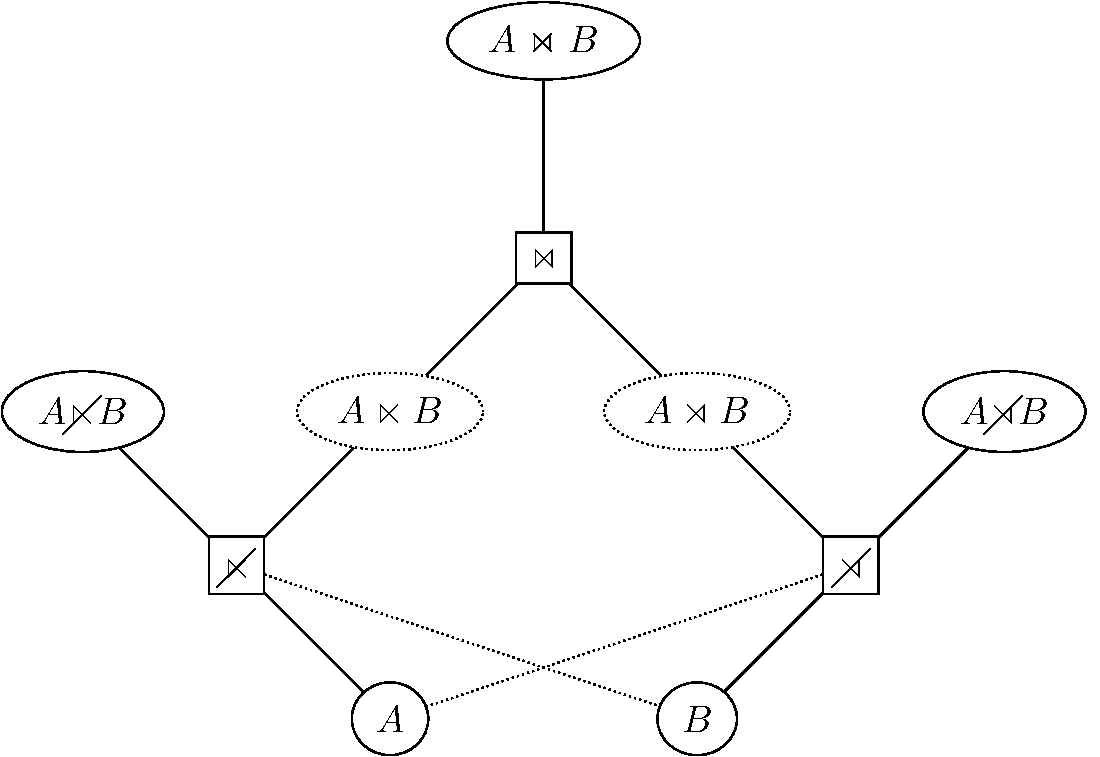
\includegraphics[width=.9\linewidth]{../imgs/joinnet.pdf}
   \end{column}
    \begin{column}{0.5\textwidth}
      \begin{tikzdiagram_w}
        \tikzset{node distance=2cm}
        \tikzset{nnode/.style={ellipse,draw}}
        \tikzset{tnode/.style={rectangle,draw}}

        \node[tnode] (t) {\(\sigma_p\)};
        \node[nnode] (o2) [above left of=t] {\(o_{sec}\)};
        \node[nnode] (o1) [above right of=t] {\(o_{prim}\)};
        \node[nnode] (i) [below of=t] {\(i\)};

        \path (t) edge (i);
        \path (t) edge (o1);
        \path (t) edge (o2);
      \end{tikzdiagram_w}
    \end{column}
  \end{columns}
\end{frame}

\begin{frame}
  \frametitle{Reversible operators}
  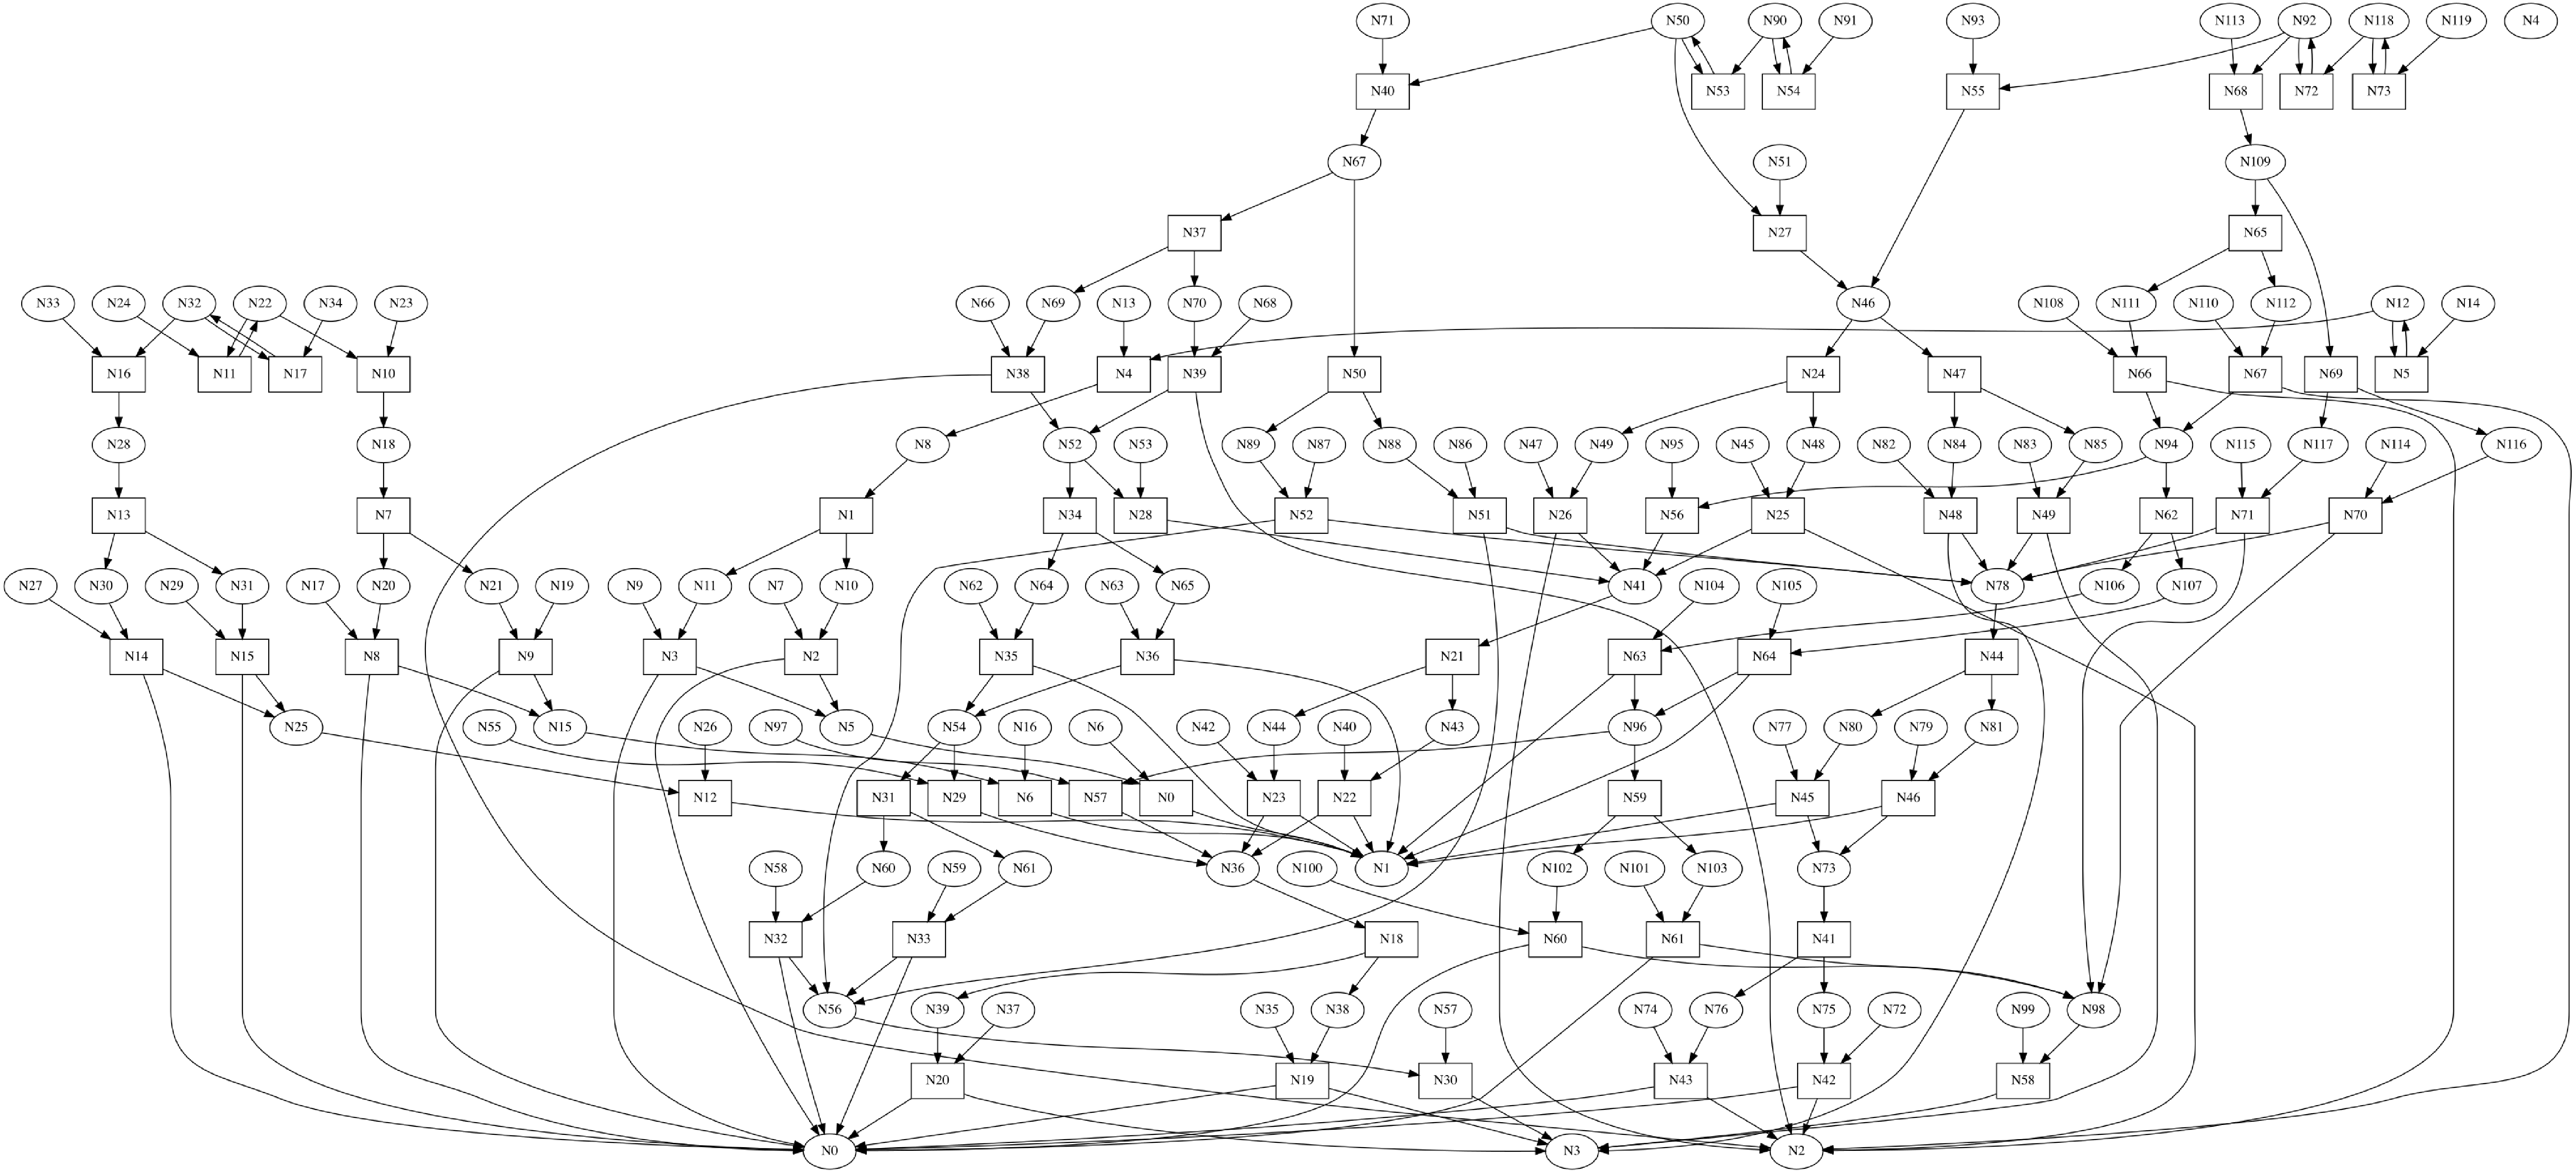
\includegraphics[width=\textwidth]{../imgs/ssb_graph.pdf}
\end{frame}



%%% Local Variables:
%%% mode: latex
%%% TeX-master: "presentation"
%%% End:
